\documentclass[a4paper,12pt]{article} % тип документа
\usepackage[margin=1in]{geometry} % Поля

%  Русский язык
\usepackage[warn]{mathtext}
\usepackage[T2A]{fontenc}			% кодировка
\usepackage[utf8]{inputenc}			% кодировка исходного текста
\usepackage[english,russian]{babel}	% локализация и переносы
% Математика
\usepackage{amsmath,amsfonts,amssymb,amsthm,mathtools} 
\usepackage{wasysym}
%%%
\usepackage{graphicx}

\usepackage{tabularx}

\usepackage{gensymb} % знак градуса
\usepackage{enumitem} % изменить список enumerate
\usepackage{placeins} % \FloatBarrier

\renewcommand{\thesection}{\Roman{section}} 
\renewcommand{\thesubsection}{\roman{subsection}}


\begin{document}

\newcolumntype{Y}{>{\centering\arraybackslash}X} %new tabularx


%титул
\hrule 	
\medskip
\begin{raggedright}
{\large \textbf{Отчёт по работе 4.7.2}}
\\
\medskip
{\Large Эффект Поккельса} 
\\
\medskip
{\large Карташов Констанин Б04-005}
\medskip
\hrule
\medskip
\end{raggedright}


\section{Анотация}

\paragraph{Цель работы:} 
Исследовать интерференцию рассеянного света, прошедшего кристалл. Наблюдать изменение характера поляризации света при наложении на кристалл электрического поля.

\paragraph{Оборудование:}
\begin{itemize}
\renewcommand{\labelitemi}{$\triangleright$}
\itemsep0em
\item He-Ne лазер,
\item Кристалл ниобата натрия,
\item Матовая пластинка,
\item Экран,
\item Лабораторный блок питания,
\item Осциллограф.
\end{itemize}


\medskip\hrule\medskip

\section{Теоретическая часть}

\subsection{Эффект Поккельса}

\paragraph{} Эффектом Поккельса называется изменение показателя преломления света в кристалле под действием электрического поля, причём это изменение пропорционально напряжённости электрического поля. Вследствие эффекта Поккельса в кристалле либо появляется двойное лучепреломление, либо меняется его величина (если кристалл был двулучепреломляющим в отсутствие поля), либо, как в данной работе, одноосный кристалл становится двуосным.

\paragraph{} Рассмотрим сначала кристалл в отсутствие внешнего электрического поля. Кристалл ниобата лития является одноосным кристаллом, то есть кристаллом, оптические свойства которого обладают симметрией вращения относительно некоторого одного направления, называемого оптической осью $z$ кристалла. Для световой волны, вектор электрического поля $E$ которой перпендикулярен оси $z$, показатель преломления равен $n_o = \sqrt{\varepsilon_\perp}$ , а для волны, вектор $E$ которой располагается вдоль оси $z$, он равен $n_e = \sqrt{\varepsilon_\parallel}$ , причём $n_e < n_o$ , т. е. LiNbO$_3$ -- <<отрицательный кристалл>>.

\paragraph{} В общем случае, когда луч света распространяется под углом $\theta$ к оптической оси $z$, существуют два собственных значения показателя преломления $n_1$ и $n_2$ : в обыкновенной волне (если световой вектор E перпендикулярен плоскости $(k, e_z )$, где $k$ — волновой вектор луча, $e_z$ -- орт по оси $z$) показатель $n_1 = n_o$ , а в необыкновенной (когда световой вектор $E$ лежит в плоскости $(k, e_z )$) показатель преломления $n_2$ зависит от угла $\theta$:

\begin{equation}
\frac{1}{n_2^2} = \frac{\cos{\theta}^2}{n_o^2} + \frac{\sin{\theta}^2}{n_e^2}.
\end{equation}

\subsection{Устройство экспериментальной установки}

\begin{figure}[h]
\centering
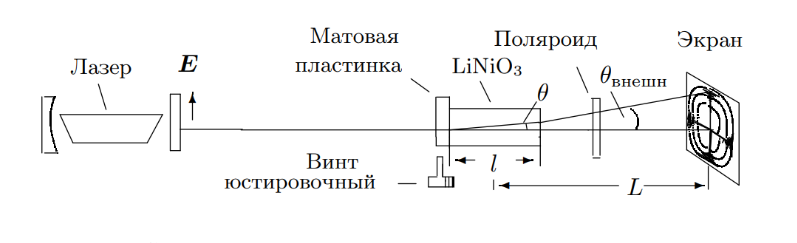
\includegraphics[width=0.8\textwidth]{setup.png}
\caption{Схема установки для наблюдения интерференционной картины}
\label{fig:setup}
\end{figure}

\begin{figure}[h]
\centering
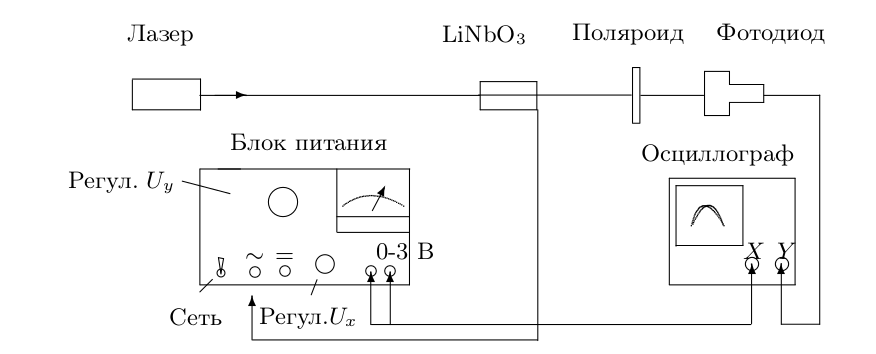
\includegraphics[width=\textwidth]{setup2.png}
\caption{Схема установки для изучения двулучепреломления в электрическом поле}
\label{fig:setup2}
\end{figure}

\paragraph{} В данной схеме свет проходит через кристалл длиной $l$ и образует интерференционную картину на экране на расстоянии $L$. Обозначим $n_0$ и $n_e$ -- коэффициенты преломления для перпендикулярной и обыкновенной волн, тогда разность фаз между обыкновенной и необыкновенной волнами равна:

\begin{equation}
\Delta \varphi = \frac{2 \pi l}{\lambda} (n_0 - n_e) \theta^2,
\label{e:deltaphi}
\end{equation}

\noindent где $\theta$ -- это угол между лучом и оптической осью z. Используя эту формулу и условие максимума можно найти радиусы образуемых на экране максимумов (внешний угол находится по закону Снеллиуса):

\begin{equation}
r^2(m) = \frac{\lambda}{l} \frac{(n_0 L)^2}{n_0 - n_e}
\label{e:rad}
\end{equation}

\paragraph{} Для изучения двулучепреломления в электрическом поле, подадим на конденсатор на кристалле напряжение с лабораторного источника питания. За поляроидом поставим фотодиод для измерения интенсивности света. Подключим выход фотодиода и блока питания к оси Y и X фотодиода соответственно, для наблюдения фигур Лиссажу. 

\medskip\hrule\medskip

\section{Экспериментальная часть}


\subsection{Наблюдение интерференционной картины}

\paragraph{} Соберём установку согласно рис. \ref{fig:setup}. Размер кристалла $3\times3\times26$ мм$^3$, коэффициент преломления $n_0=2.29$, длина волны $\lambda = 0.63$ мкм, расстояние от экрана до центра кристалла $L = 70.5 \pm 1$ см.

\paragraph{} Исследуем зависимость радиуса интерференционных колец от их порядка. Данные измерений запишем в таблицу \ref{tab:radius}. Оценим погрешность измерения радиусов колец через половину их толщины: $\sigma_r \approx 1$ мм, а значит $\sigma_{r^2} = 2r \cdot \sigma_r$ мм.

\begin{table}[h]
\centering
\begin{tabular}{|l|l|l|l|l|l|l|l|l|l|l|l|}
\hline
$m$           & 1   & 2    & 3    & 4    & 5    & 6    & 7    & 8    & 9    & 10   & 11   \\ \hline
$r$, мм       & 27  & 39   & 47   & 54   & 60   & 67   & 71   & 76   & 81   & 84   & 88   \\ \hline
$r^2$, мм$^2$ & 729 & 1521 & 2209 & 2916 & 3600 & 4489 & 4041 & 5776 & 6561 & 7056 & 7744 \\ \hline
\end{tabular}
\caption{Зависимость радиусов интерференционных колец от их порядка}
\label{tab:radius}
\end{table}

\paragraph{} По данным из из таблицы \ref{tab:radius} построим график зависимости $r^2(n)$. Пользуясь методом наименьших квадратов проведём наилучшую прямую (рис. \ref{fig:plot}). Получаем $\partial r^2 / \partial m = \alpha = 713 \pm 7$ мм.

\begin{figure}[h]
\centering
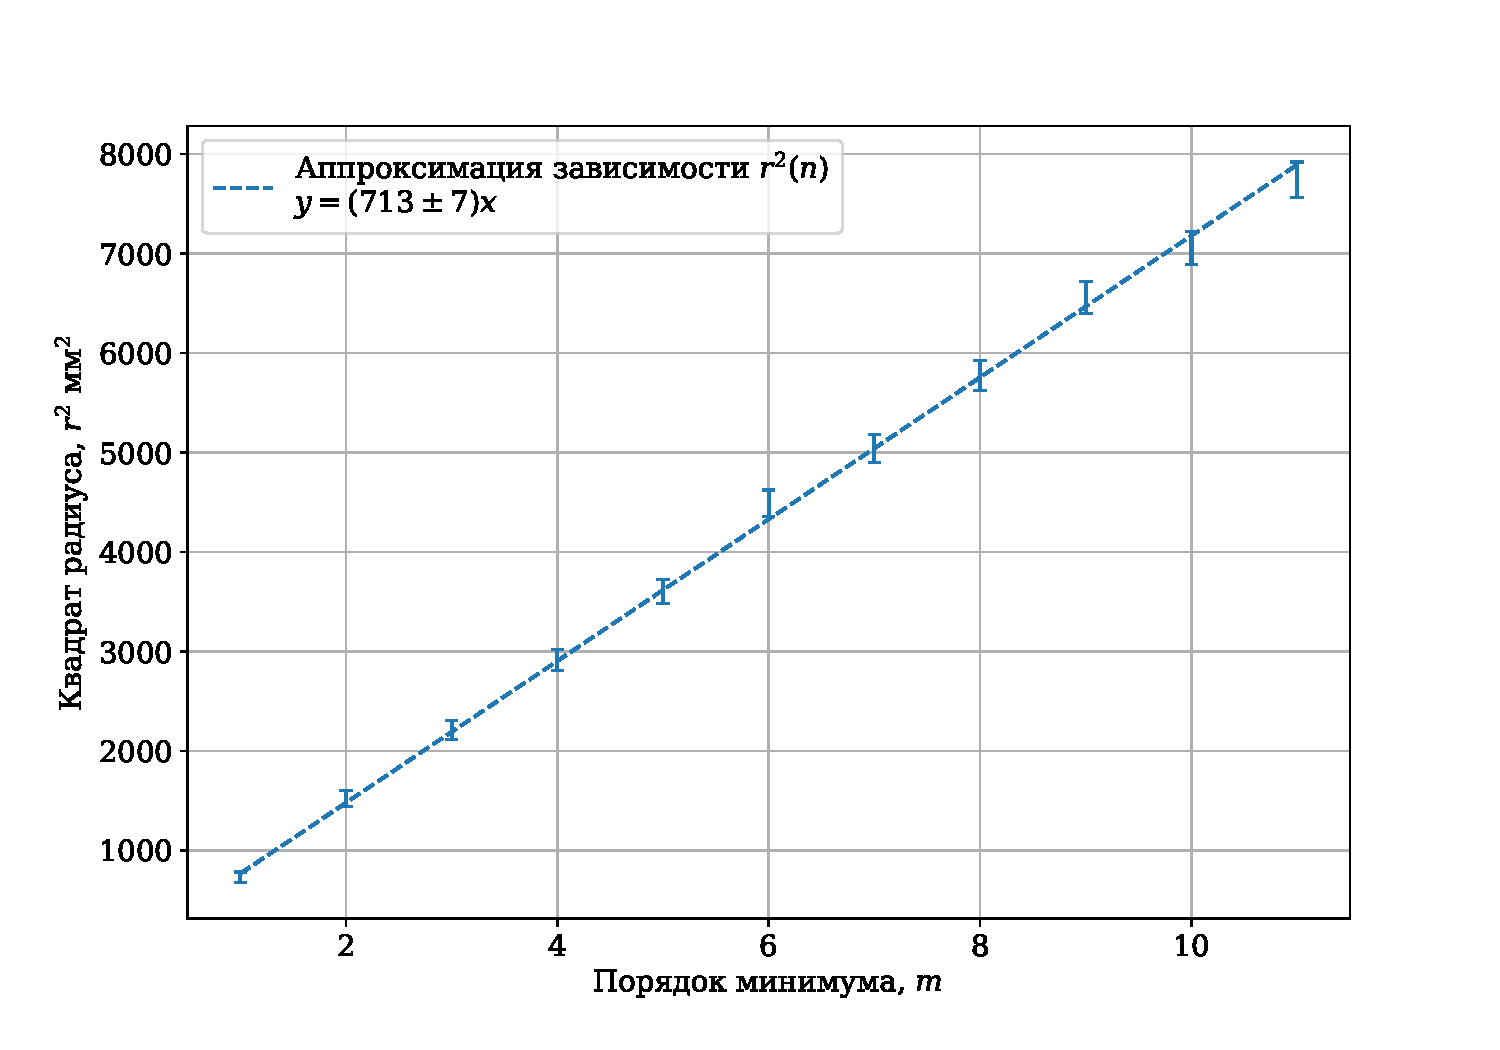
\includegraphics[width=\textwidth]{plot.pdf}
\caption{График зависимости $r^2(n)$}
\label{fig:plot}
\end{figure}

\paragraph{} Пользуясь формулой (\ref{e:rad}) найдём значение $n_o - n_e$:

\[
\delta n = n_o - n_e = \frac{\lambda (n_0 L)^2}{l} \frac{\partial m}{\partial r^2} = \frac{\lambda (n_0 L)^2}{l \alpha} = \frac{0.63 \cdot 10^{-3} \cdot (2.29 \cdot 705)^2}{26 \cdot 713} = 0.089,
\]\[
\sigma_{\delta n} = \delta n \sqrt{4\left( \frac{\sigma_L}{L} \right)^2 + \left( \frac{\sigma_\alpha}{\alpha} \right)^2} = 0.089 \sqrt{4\left( \frac{1}{70.5} \right)^2 + \left( \frac{7}{713} \right)^2} = 0.003.
\]

\noindent Получаем $\delta n = 0.089 \pm 0.003$.

\subsection{Изучение оптический свойств кристалла в электрическом поле}

\paragraph{} Включим лабораторный блок питания и выстави режим постоянного тока, уберём матовую пластинку. Меняя напряжение найдём положение в котором яркость пятна будет максимальным -- это полуволновое напряжение. Так как точное положение максимальной яркости сложно определить на глаз, измеренное значение полуволнового напряжение -- интервал в котором яркость заметно не меняется. Измеренное полуволновое напряжение $U_{\lambda / 2} = 0.45 \div 0.54$ кВ. 

\paragraph{} Проделаем тот же опыт при параллельных осях поляризаторов. Теперь при полуволновом напряжении яркость будет минимальной. Измеренное $U_{\lambda / 2} = 0.45 \div 0.54$ кВ -- такое же как и в прошлом случае.

\paragraph{} Подадим на кристалл четвертьволновое напряжение $U_{\lambda / 4} = U_{\lambda / 2} / 2$. При вращении поляризатора, яркость пятна не меняется -- значит поляризация света круговая.

\paragraph{} Выставим на блоке питания режим переменного тока, поставим по ходу луча фотодиод, включим осциллограф, подадим на ось X -- напряжение блока питания, на ость Y -- напряжение фотодиода (рис. \ref{fig:setup2}). На экране осциллографа пронаблюдаем видны синусоидальные фигуры Лиссажу, при увеличении амплитуды напряжения -- увеличивается количество периодов в фигуре Лиссажу. 

\paragraph{} Фигуры для различных значений напряжения изображены на рис. \ref{fig:per1}, \ref{fig:per2}, \ref{fig:per3}. По фигуре Лиссажу определим $U_{\lambda/2} = 0.44 \pm 0.02$ кВ. Погрешность определяем по цене деления на блоке питания. 


\begin{figure}
\centering
\begin{minipage}{0.49\textwidth}
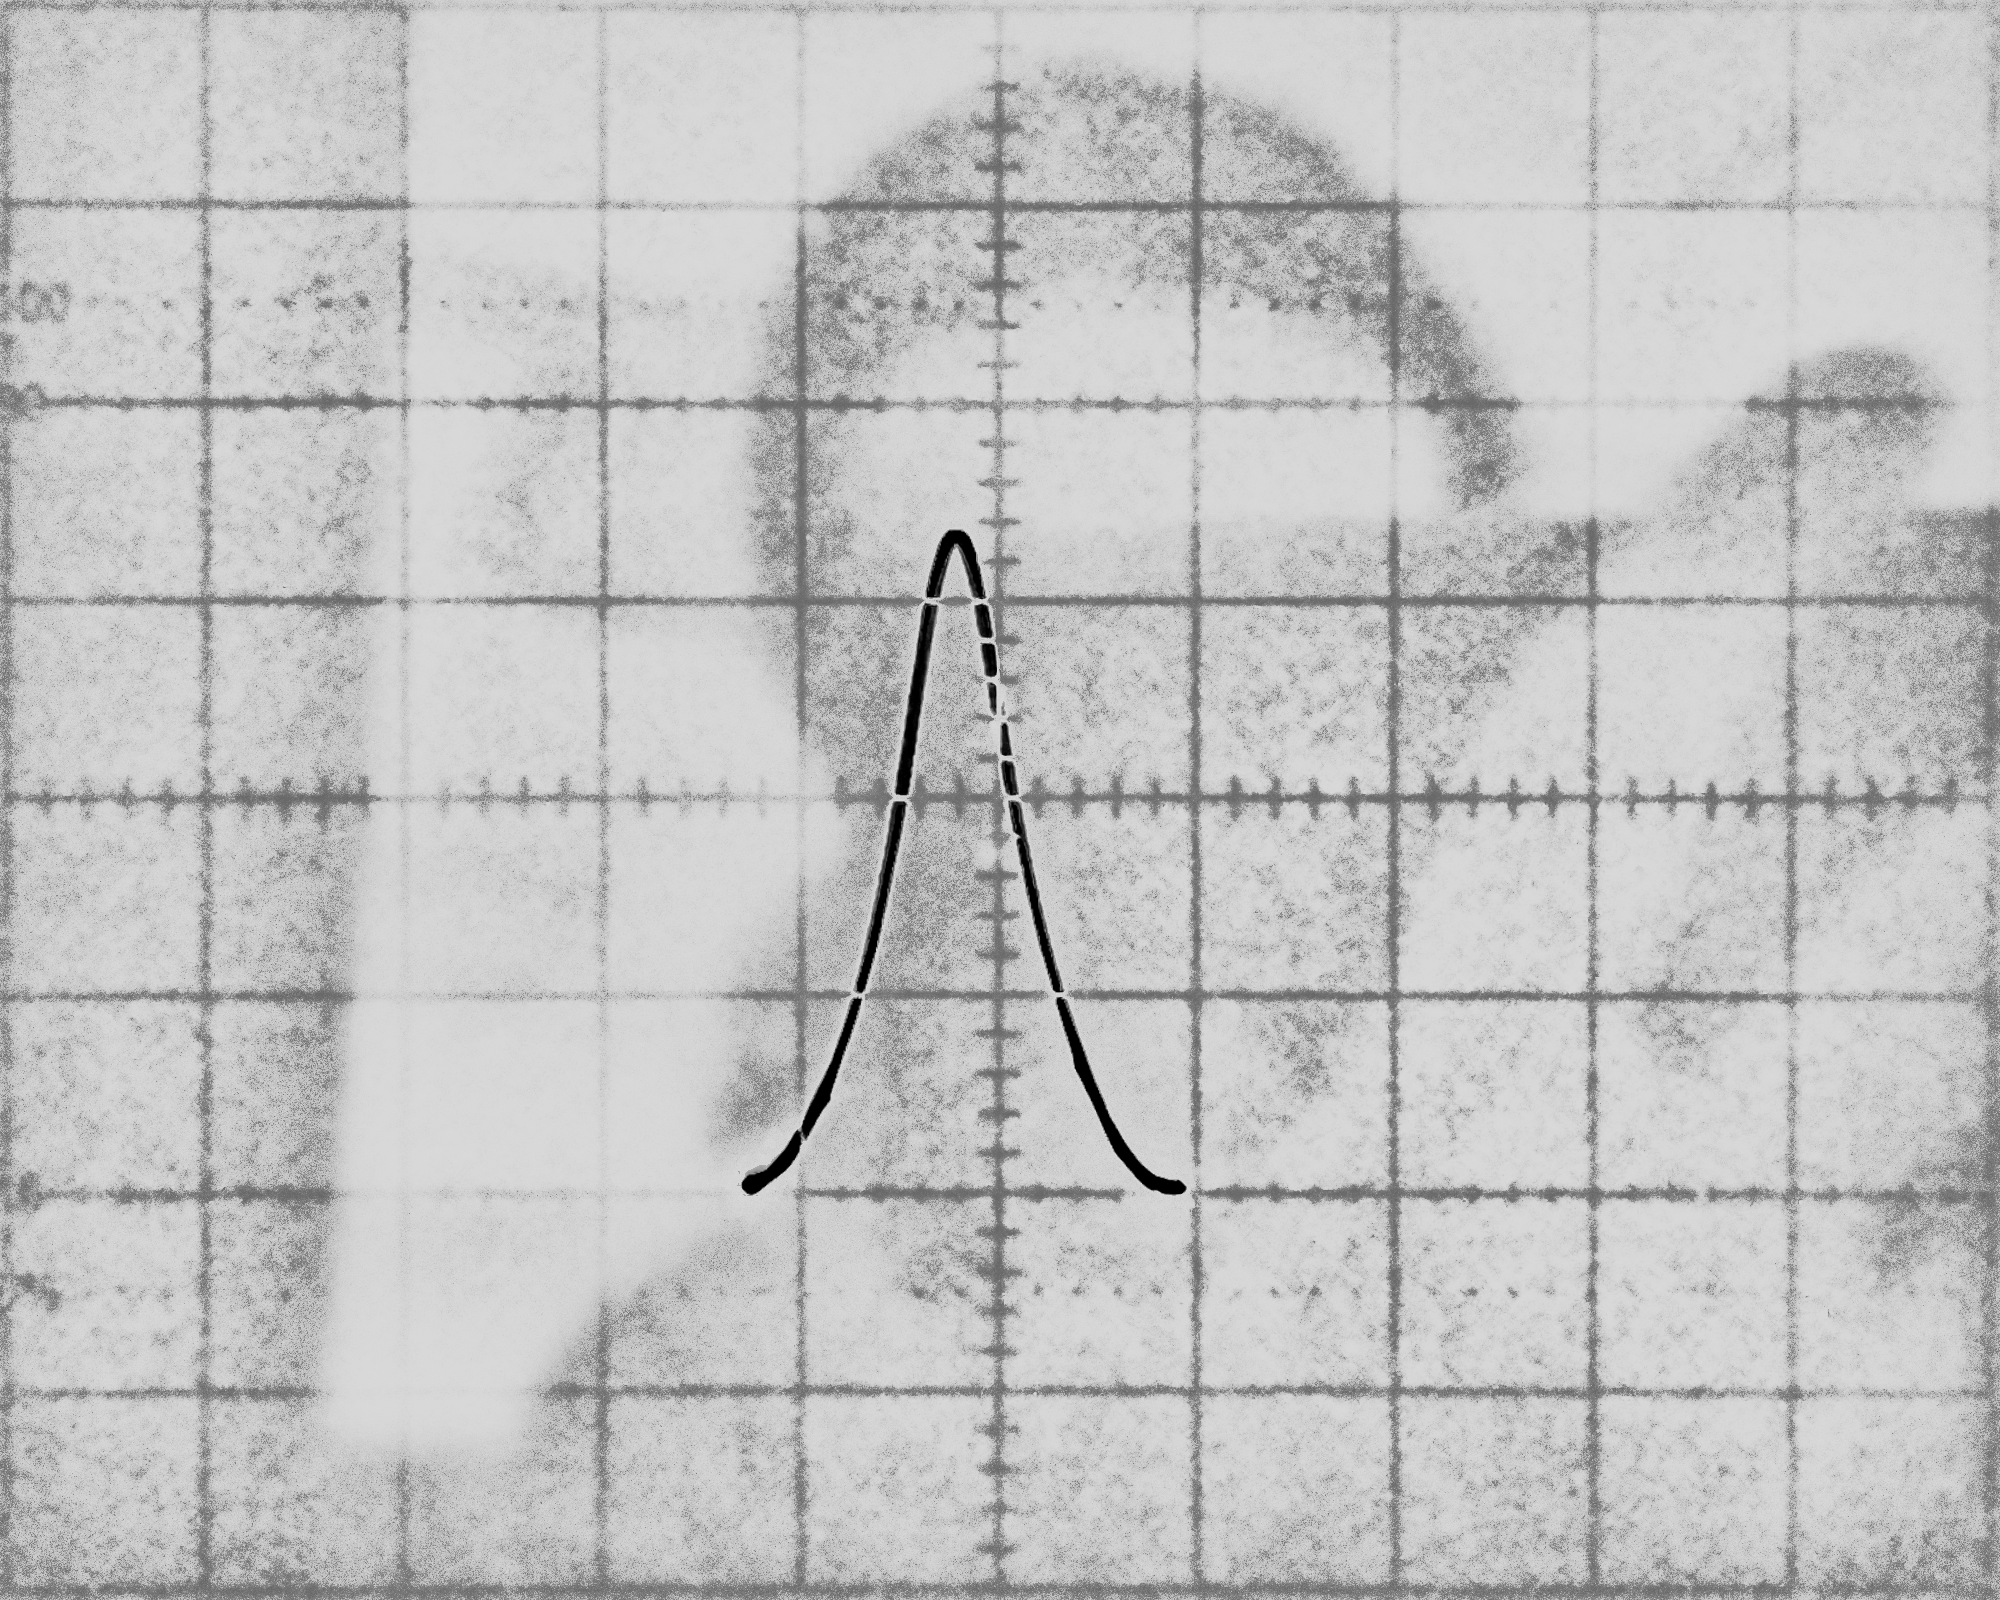
\includegraphics[width=0.9\textwidth]{1per.png}
\caption{Фигура Лиссажу для $U_{\lambda/2}$}
\label{fig:per1}
\end{minipage}
\begin{minipage}{0.49\textwidth}
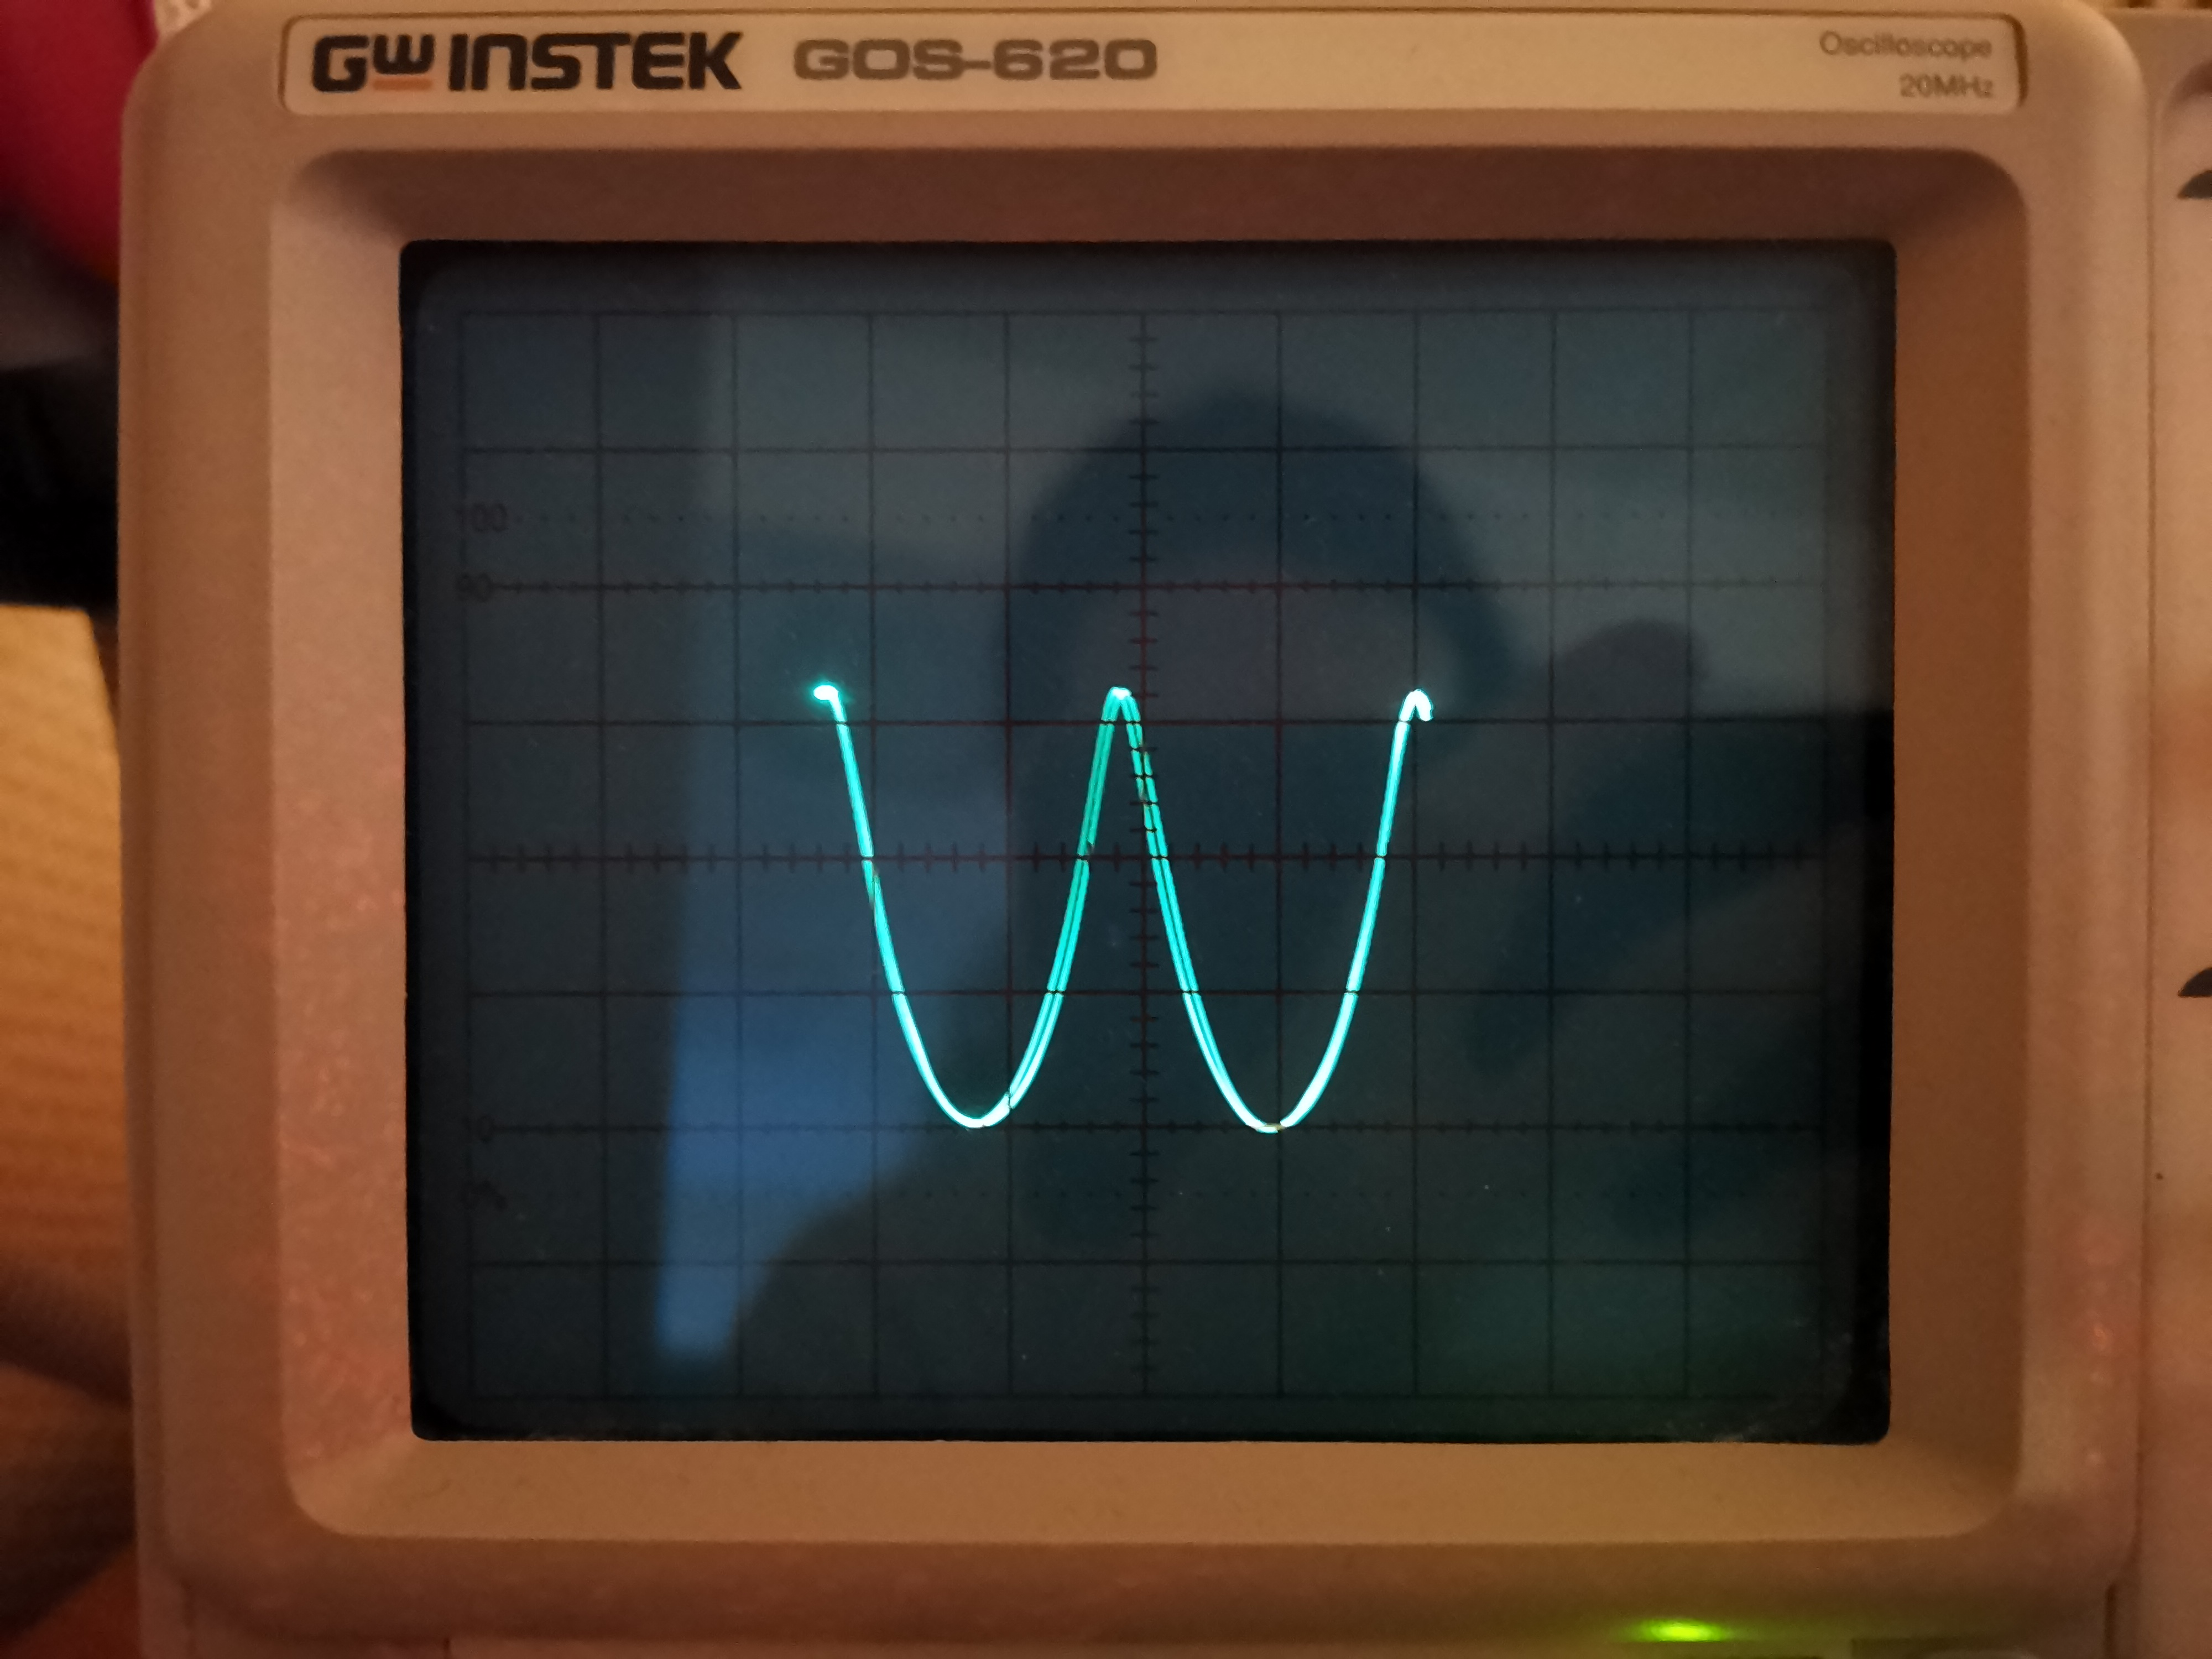
\includegraphics[width=0.9\textwidth]{2per.png}
\caption{Фигура Лиссажу для $U_{\lambda}$}
\label{fig:per2}
\end{minipage}
\medskip\medskip
\begin{minipage}{0.49\textwidth}
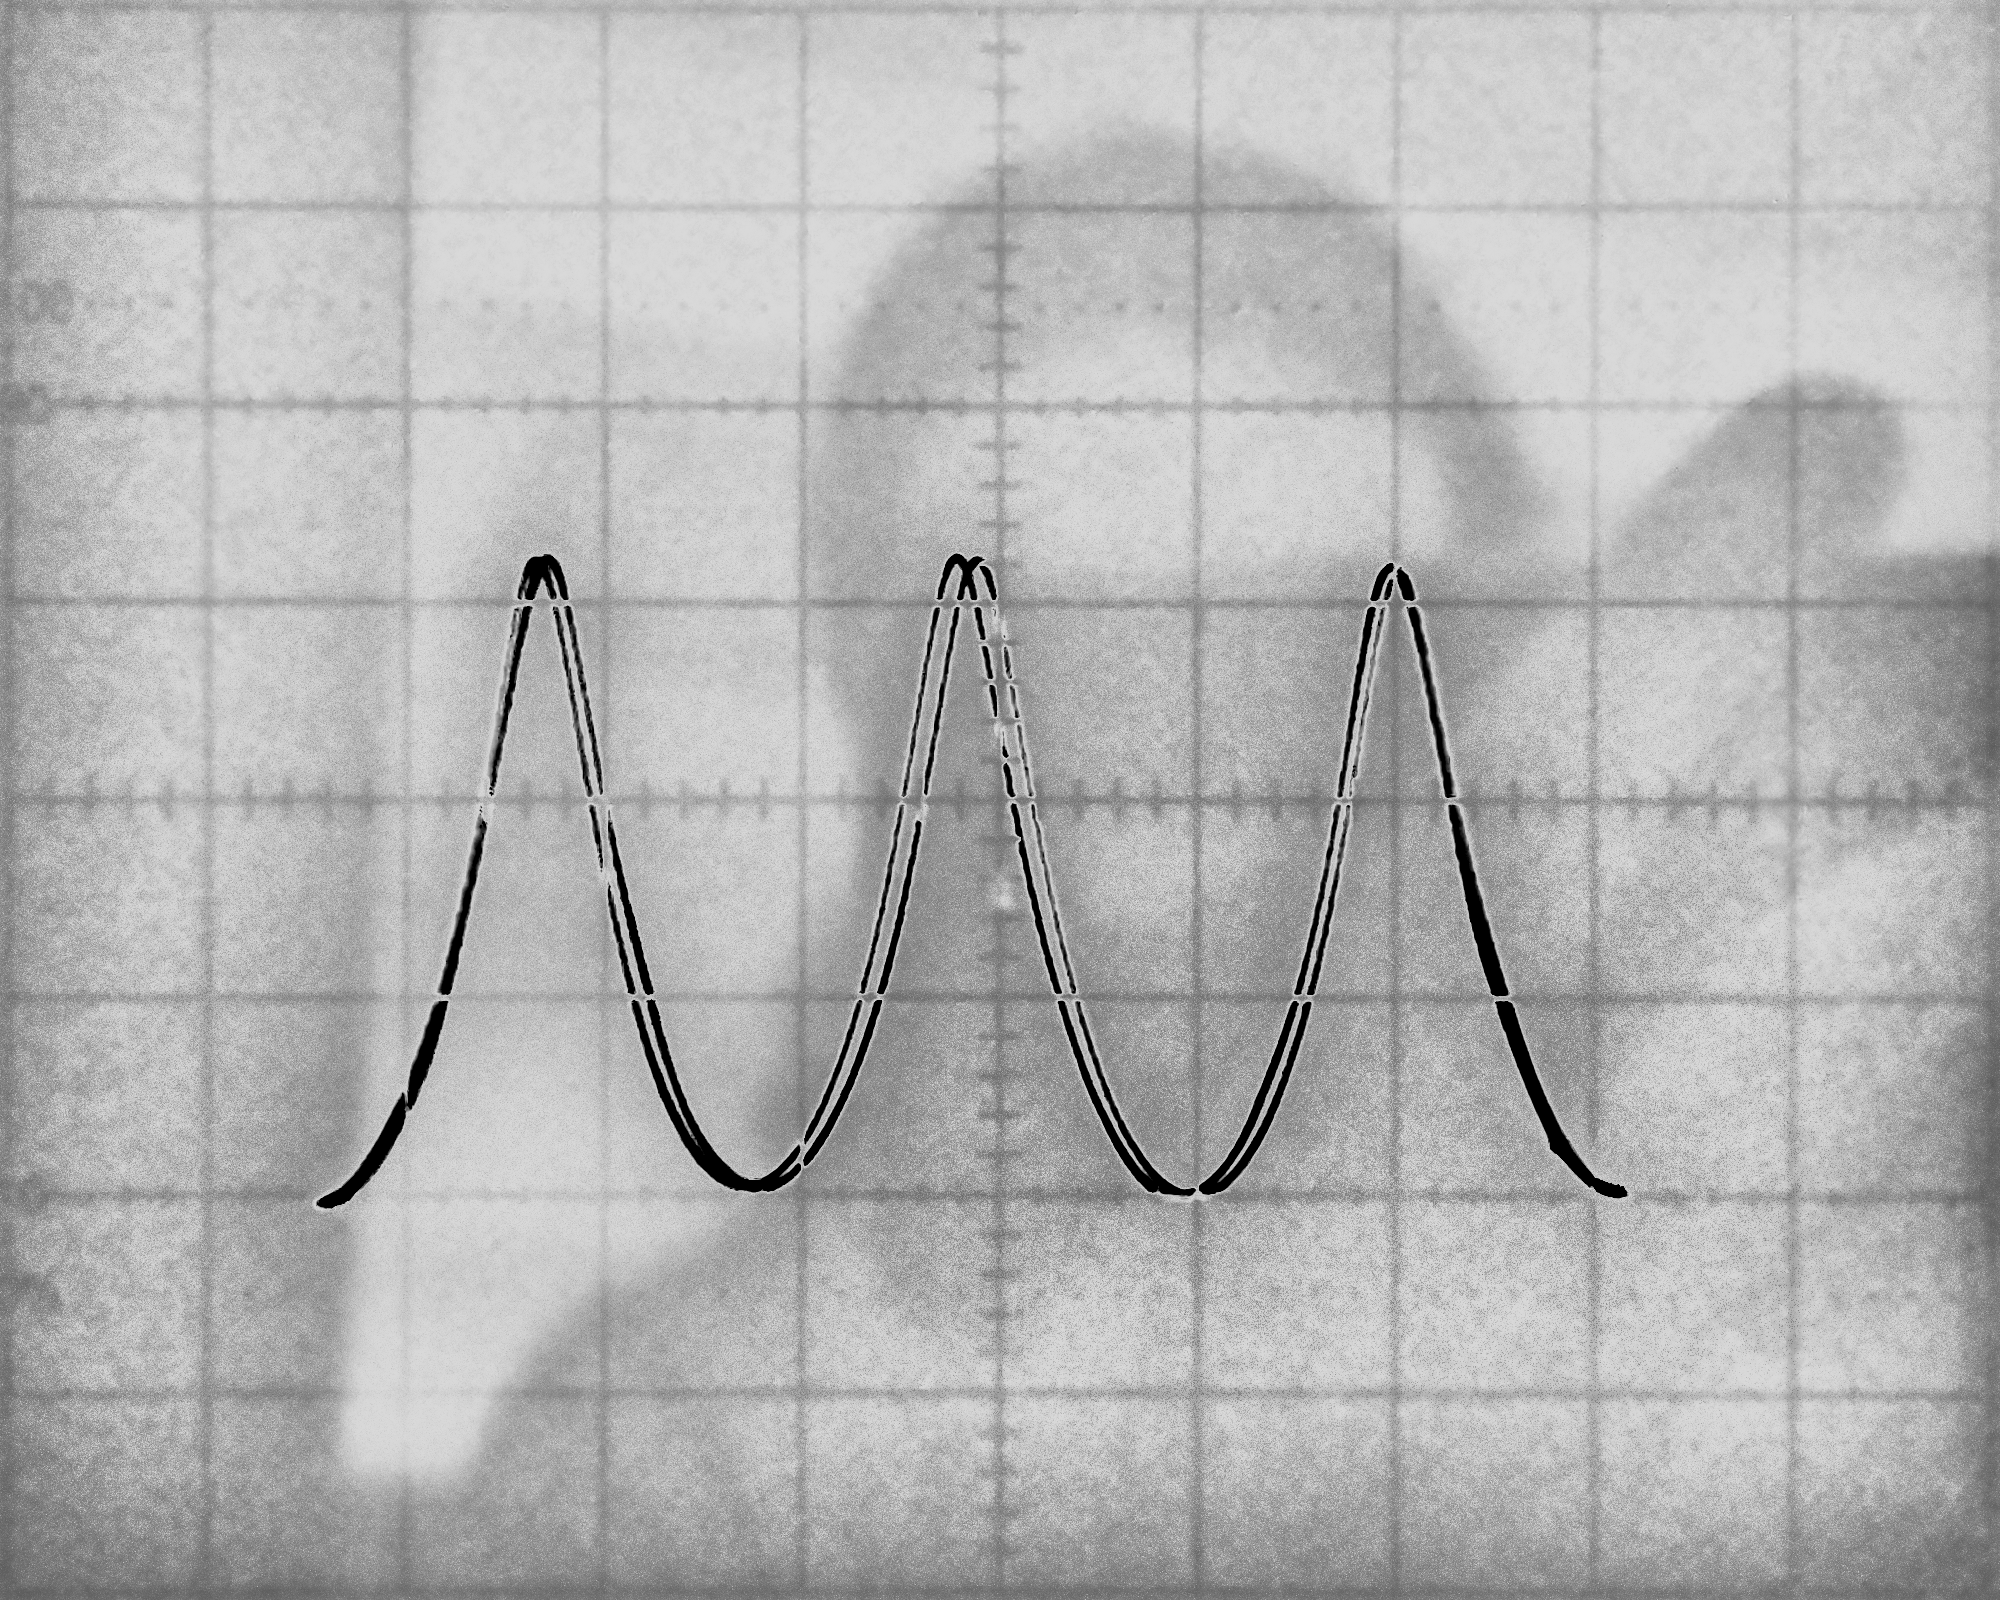
\includegraphics[width=0.9\textwidth]{3per.png}
\caption{Фигура Лиссажу для $U_{3\lambda/2}$}
\label{fig:per3}
\end{minipage}
\end{figure}


\medskip\hrule\medskip

\section{Выводы}

\begin{enumerate}
\item Пронаблюдали эффект двулучепреломления в кристалле. Через радиусы колец интерференционной картины определили значение двулучепреломления ниобата лития: $\delta n = 0.089 \pm 0.003$
\item Пронаблюдали эффект Поккельса, подавая напряжение на кристалл. Измерили напряжение при котором кристалл ведёт сея как пластинка $\lambda /2$. $U_{\lambda / 2} = 0.44 \pm 2$ кВ.
\end{enumerate}

\medskip\hrule\medskip

\end{document}
